% Options for packages loaded elsewhere
\PassOptionsToPackage{unicode}{hyperref}
\PassOptionsToPackage{hyphens}{url}
\PassOptionsToPackage{dvipsnames,svgnames,x11names}{xcolor}
%
\documentclass[
  letterpaper,
  DIV=11,
  numbers=noendperiod]{scrreprt}

\usepackage{amsmath,amssymb}
\usepackage{iftex}
\ifPDFTeX
  \usepackage[T1]{fontenc}
  \usepackage[utf8]{inputenc}
  \usepackage{textcomp} % provide euro and other symbols
\else % if luatex or xetex
  \usepackage{unicode-math}
  \defaultfontfeatures{Scale=MatchLowercase}
  \defaultfontfeatures[\rmfamily]{Ligatures=TeX,Scale=1}
\fi
\usepackage{lmodern}
\ifPDFTeX\else  
    % xetex/luatex font selection
\fi
% Use upquote if available, for straight quotes in verbatim environments
\IfFileExists{upquote.sty}{\usepackage{upquote}}{}
\IfFileExists{microtype.sty}{% use microtype if available
  \usepackage[]{microtype}
  \UseMicrotypeSet[protrusion]{basicmath} % disable protrusion for tt fonts
}{}
\makeatletter
\@ifundefined{KOMAClassName}{% if non-KOMA class
  \IfFileExists{parskip.sty}{%
    \usepackage{parskip}
  }{% else
    \setlength{\parindent}{0pt}
    \setlength{\parskip}{6pt plus 2pt minus 1pt}}
}{% if KOMA class
  \KOMAoptions{parskip=half}}
\makeatother
\usepackage{xcolor}
\setlength{\emergencystretch}{3em} % prevent overfull lines
\setcounter{secnumdepth}{5}
% Make \paragraph and \subparagraph free-standing
\ifx\paragraph\undefined\else
  \let\oldparagraph\paragraph
  \renewcommand{\paragraph}[1]{\oldparagraph{#1}\mbox{}}
\fi
\ifx\subparagraph\undefined\else
  \let\oldsubparagraph\subparagraph
  \renewcommand{\subparagraph}[1]{\oldsubparagraph{#1}\mbox{}}
\fi

\usepackage{color}
\usepackage{fancyvrb}
\newcommand{\VerbBar}{|}
\newcommand{\VERB}{\Verb[commandchars=\\\{\}]}
\DefineVerbatimEnvironment{Highlighting}{Verbatim}{commandchars=\\\{\}}
% Add ',fontsize=\small' for more characters per line
\usepackage{framed}
\definecolor{shadecolor}{RGB}{241,243,245}
\newenvironment{Shaded}{\begin{snugshade}}{\end{snugshade}}
\newcommand{\AlertTok}[1]{\textcolor[rgb]{0.68,0.00,0.00}{#1}}
\newcommand{\AnnotationTok}[1]{\textcolor[rgb]{0.37,0.37,0.37}{#1}}
\newcommand{\AttributeTok}[1]{\textcolor[rgb]{0.40,0.45,0.13}{#1}}
\newcommand{\BaseNTok}[1]{\textcolor[rgb]{0.68,0.00,0.00}{#1}}
\newcommand{\BuiltInTok}[1]{\textcolor[rgb]{0.00,0.23,0.31}{#1}}
\newcommand{\CharTok}[1]{\textcolor[rgb]{0.13,0.47,0.30}{#1}}
\newcommand{\CommentTok}[1]{\textcolor[rgb]{0.37,0.37,0.37}{#1}}
\newcommand{\CommentVarTok}[1]{\textcolor[rgb]{0.37,0.37,0.37}{\textit{#1}}}
\newcommand{\ConstantTok}[1]{\textcolor[rgb]{0.56,0.35,0.01}{#1}}
\newcommand{\ControlFlowTok}[1]{\textcolor[rgb]{0.00,0.23,0.31}{#1}}
\newcommand{\DataTypeTok}[1]{\textcolor[rgb]{0.68,0.00,0.00}{#1}}
\newcommand{\DecValTok}[1]{\textcolor[rgb]{0.68,0.00,0.00}{#1}}
\newcommand{\DocumentationTok}[1]{\textcolor[rgb]{0.37,0.37,0.37}{\textit{#1}}}
\newcommand{\ErrorTok}[1]{\textcolor[rgb]{0.68,0.00,0.00}{#1}}
\newcommand{\ExtensionTok}[1]{\textcolor[rgb]{0.00,0.23,0.31}{#1}}
\newcommand{\FloatTok}[1]{\textcolor[rgb]{0.68,0.00,0.00}{#1}}
\newcommand{\FunctionTok}[1]{\textcolor[rgb]{0.28,0.35,0.67}{#1}}
\newcommand{\ImportTok}[1]{\textcolor[rgb]{0.00,0.46,0.62}{#1}}
\newcommand{\InformationTok}[1]{\textcolor[rgb]{0.37,0.37,0.37}{#1}}
\newcommand{\KeywordTok}[1]{\textcolor[rgb]{0.00,0.23,0.31}{#1}}
\newcommand{\NormalTok}[1]{\textcolor[rgb]{0.00,0.23,0.31}{#1}}
\newcommand{\OperatorTok}[1]{\textcolor[rgb]{0.37,0.37,0.37}{#1}}
\newcommand{\OtherTok}[1]{\textcolor[rgb]{0.00,0.23,0.31}{#1}}
\newcommand{\PreprocessorTok}[1]{\textcolor[rgb]{0.68,0.00,0.00}{#1}}
\newcommand{\RegionMarkerTok}[1]{\textcolor[rgb]{0.00,0.23,0.31}{#1}}
\newcommand{\SpecialCharTok}[1]{\textcolor[rgb]{0.37,0.37,0.37}{#1}}
\newcommand{\SpecialStringTok}[1]{\textcolor[rgb]{0.13,0.47,0.30}{#1}}
\newcommand{\StringTok}[1]{\textcolor[rgb]{0.13,0.47,0.30}{#1}}
\newcommand{\VariableTok}[1]{\textcolor[rgb]{0.07,0.07,0.07}{#1}}
\newcommand{\VerbatimStringTok}[1]{\textcolor[rgb]{0.13,0.47,0.30}{#1}}
\newcommand{\WarningTok}[1]{\textcolor[rgb]{0.37,0.37,0.37}{\textit{#1}}}

\providecommand{\tightlist}{%
  \setlength{\itemsep}{0pt}\setlength{\parskip}{0pt}}\usepackage{longtable,booktabs,array}
\usepackage{calc} % for calculating minipage widths
% Correct order of tables after \paragraph or \subparagraph
\usepackage{etoolbox}
\makeatletter
\patchcmd\longtable{\par}{\if@noskipsec\mbox{}\fi\par}{}{}
\makeatother
% Allow footnotes in longtable head/foot
\IfFileExists{footnotehyper.sty}{\usepackage{footnotehyper}}{\usepackage{footnote}}
\makesavenoteenv{longtable}
\usepackage{graphicx}
\makeatletter
\def\maxwidth{\ifdim\Gin@nat@width>\linewidth\linewidth\else\Gin@nat@width\fi}
\def\maxheight{\ifdim\Gin@nat@height>\textheight\textheight\else\Gin@nat@height\fi}
\makeatother
% Scale images if necessary, so that they will not overflow the page
% margins by default, and it is still possible to overwrite the defaults
% using explicit options in \includegraphics[width, height, ...]{}
\setkeys{Gin}{width=\maxwidth,height=\maxheight,keepaspectratio}
% Set default figure placement to htbp
\makeatletter
\def\fps@figure{htbp}
\makeatother

\KOMAoption{captions}{tableheading}
\makeatletter
\makeatother
\makeatletter
\@ifpackageloaded{bookmark}{}{\usepackage{bookmark}}
\makeatother
\makeatletter
\@ifpackageloaded{caption}{}{\usepackage{caption}}
\AtBeginDocument{%
\ifdefined\contentsname
  \renewcommand*\contentsname{Table of contents}
\else
  \newcommand\contentsname{Table of contents}
\fi
\ifdefined\listfigurename
  \renewcommand*\listfigurename{List of Figures}
\else
  \newcommand\listfigurename{List of Figures}
\fi
\ifdefined\listtablename
  \renewcommand*\listtablename{List of Tables}
\else
  \newcommand\listtablename{List of Tables}
\fi
\ifdefined\figurename
  \renewcommand*\figurename{Figure}
\else
  \newcommand\figurename{Figure}
\fi
\ifdefined\tablename
  \renewcommand*\tablename{Table}
\else
  \newcommand\tablename{Table}
\fi
}
\@ifpackageloaded{float}{}{\usepackage{float}}
\floatstyle{ruled}
\@ifundefined{c@chapter}{\newfloat{codelisting}{h}{lop}}{\newfloat{codelisting}{h}{lop}[chapter]}
\floatname{codelisting}{Listing}
\newcommand*\listoflistings{\listof{codelisting}{List of Listings}}
\makeatother
\makeatletter
\@ifpackageloaded{caption}{}{\usepackage{caption}}
\@ifpackageloaded{subcaption}{}{\usepackage{subcaption}}
\makeatother
\makeatletter
\@ifpackageloaded{tcolorbox}{}{\usepackage[skins,breakable]{tcolorbox}}
\makeatother
\makeatletter
\@ifundefined{shadecolor}{\definecolor{shadecolor}{rgb}{.97, .97, .97}}
\makeatother
\makeatletter
\makeatother
\makeatletter
\makeatother
\ifLuaTeX
  \usepackage{selnolig}  % disable illegal ligatures
\fi
\IfFileExists{bookmark.sty}{\usepackage{bookmark}}{\usepackage{hyperref}}
\IfFileExists{xurl.sty}{\usepackage{xurl}}{} % add URL line breaks if available
\urlstyle{same} % disable monospaced font for URLs
\hypersetup{
  pdftitle={Github tutorial},
  pdfauthor={Sarah Endicott},
  colorlinks=true,
  linkcolor={blue},
  filecolor={Maroon},
  citecolor={Blue},
  urlcolor={Blue},
  pdfcreator={LaTeX via pandoc}}

\title{Github tutorial}
\author{Sarah Endicott}
\date{2023-06-02}

\begin{document}
\maketitle
\ifdefined\Shaded\renewenvironment{Shaded}{\begin{tcolorbox}[breakable, sharp corners, interior hidden, boxrule=0pt, borderline west={3pt}{0pt}{shadecolor}, enhanced, frame hidden]}{\end{tcolorbox}}\fi

\renewcommand*\contentsname{Table of contents}
{
\hypersetup{linkcolor=}
\setcounter{tocdepth}{2}
\tableofcontents
}
\bookmarksetup{startatroot}

\hypertarget{using-github-for-reproducible-research}{%
\chapter*{Using GitHub for Reproducible
Research}\label{using-github-for-reproducible-research}}
\addcontentsline{toc}{chapter}{Using GitHub for Reproducible Research}

\markboth{Using GitHub for Reproducible Research}{Using GitHub for
Reproducible Research}

This contains a set of tutorials for setting up and learning to use Git
and GitHub with R and RStudio. It borrows heavily from
\href{https://happygitwithr.com/index.html}{Happy Git With R} by Jenny
Bryan but with less details.

\bookmarksetup{startatroot}

\hypertarget{installation-and-setup}{%
\chapter{Installation and Setup}\label{installation-and-setup}}

\hypertarget{installation}{%
\section{Installation}\label{installation}}

\begin{itemize}
\item
  Install R and Rstudio (available from ECCC Software Centre)

  \begin{itemize}
  \tightlist
  \item
    Software Centre can be very slow to install, you can install R and
    RStudio without administrator permissions from the internet as well
    \url{https://posit.co/download/rstudio-desktop/}
  \end{itemize}
\item
  Install Git \url{https://gitforwindows.org/} (does not require admin
  permissions)

  \begin{itemize}
  \tightlist
  \item
    NOTE: When asked about ``Adjusting your PATH environment'', make
    sure to select ``Git from the command line and also from 3rd-party
    software''. Otherwise, accept the defaults.
  \end{itemize}
\item
  Create a GitHub account \url{https://github.com/}
\item
  Install R packages: Open RStudio and run in the console:

  \begin{itemize}
  \tightlist
  \item
    \texttt{install.packages("usethis")}
  \item
    \texttt{install.packages("gitcreds")}
  \end{itemize}
\end{itemize}

\hypertarget{set-username-and-email-for-git}{%
\section{Set username and email for
git}\label{set-username-and-email-for-git}}

\begin{itemize}
\tightlist
\item
  \texttt{usethis::use\_git\_config(user.name\ =\ "Jane\ Doe",\ user.email\ =\ "jane@example.org")}

  \begin{itemize}
  \tightlist
  \item
    \texttt{user.name} is the name associated with your git commits so
    just make it informative for your collaborators (ie: actual name,
    github username)
  \item
    \texttt{user.email} must match your GitHub account email
  \end{itemize}
\end{itemize}

\hypertarget{let-git-talk-to-github}{%
\section{Let git talk to GitHub}\label{let-git-talk-to-github}}

\begin{itemize}
\tightlist
\item
  \texttt{usethis::create\_github\_token()}

  \begin{itemize}
  \tightlist
  \item
    Opens GitHub webpage: select ``repo'' (always selected so it is
    greyed out), ``user'', and ``workflow'' scopes.
  \item
    Copy the token
  \end{itemize}
\item
  \texttt{gitcreds::gitcreds\_set()}

  \begin{itemize}
  \tightlist
  \item
    Should prompt you to paste your token and it will store it in the
    git credential manager.
  \end{itemize}
\end{itemize}

\hypertarget{start-a-new-project-with-github}{%
\section{Start a new project with
GitHub}\label{start-a-new-project-with-github}}

\textbf{Step 1}: Make a new repo on GitHub

\begin{itemize}
\item
  Go to \url{https://github.com} and make sure you are logged in.
\item
  Near ``Repositories'', click the big green ``New'' button.

  \begin{itemize}
  \tightlist
  \item
    How to fill this in:

    \begin{itemize}
    \tightlist
    \item
      Repository template: No template.
    \item
      Repository name: myrepo . Like a variable name, in code:
      descriptive but brief, no whitespace. Letters, digits, - , . , or
      \_ are allowed.
    \item
      Description: any short description of the project
    \item
      Public.
    \item
      Initialize this repository with: Add a README file.
    \item
      Click the big green button that says ``Create repository''.
    \end{itemize}
  \end{itemize}
\end{itemize}

\textbf{Step 2}: Copy repo URL

\begin{itemize}
\item
  Now click the big green button that says ``\textless\textgreater{}
  Code''.
\item
  Copy a clone URL to your clipboard. Use the HTTPS URL.
\end{itemize}

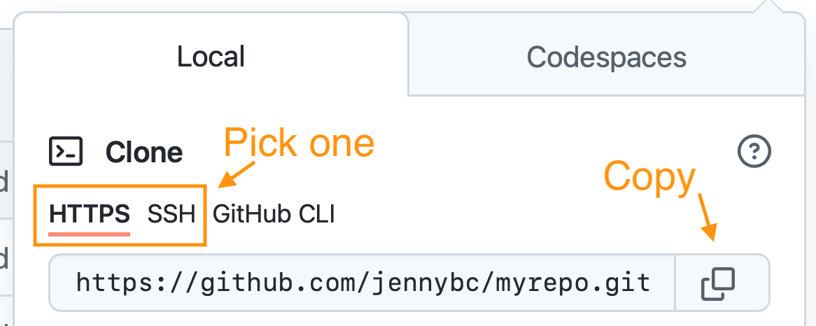
\includegraphics{assets/img/clone_url.png}

\textbf{Step 3}: Clone into a new project in RStudio

\begin{itemize}
\tightlist
\item
  File \textgreater{} New Project \textgreater{} Version Control
  \textgreater{} Git. In the ``repository URL'' paste the URL of your
  new GitHub repository.

  \begin{itemize}
  \tightlist
  \item
    Be intentional about where you create this Project. Don't put it
    inside another git repository.
  \item
    I suggest you ``Open in new session''.
  \end{itemize}
\item
  Click ``Create Project'' to create a new directory,
\item
  This should download the README.md file that we created on GitHub in
  the previous step. Look in RStudio's file browser pane for the
  README.md file.
\item
  Behind the scenes, RStudio has done this for you:
  \texttt{git\ clone\ https://github.com/see24/myrepo.git}
\end{itemize}

\hypertarget{work-on-a-project}{%
\section{Work on a project}\label{work-on-a-project}}

\begin{itemize}
\tightlist
\item
  Edit the README.md file, e.g., by adding the line ``This is a line
  from RStudio''.
\item
  Save the file locally
\item
  On the Git pane click commit
\end{itemize}

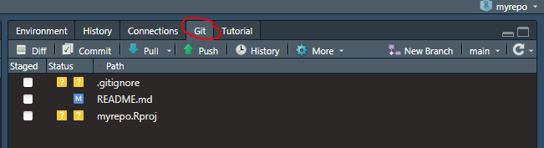
\includegraphics{assets/img/git_pane.png}

\begin{itemize}
\tightlist
\item
  In the pop-up review the changes at the bottom
\item
  Check the ``Staged'' box and type a commit message and click
  ``Commit''
\end{itemize}

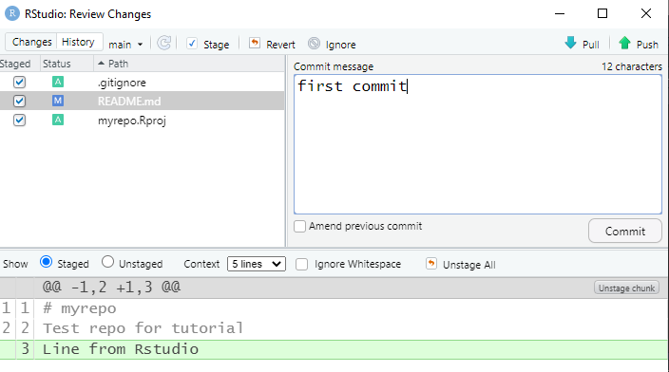
\includegraphics{assets/img/git_commit_modal.png}

\hypertarget{sync-changes-to-github-push}{%
\subsection{Sync changes to GitHub:
Push}\label{sync-changes-to-github-push}}

\begin{itemize}
\tightlist
\item
  Click ``Push'' in the Rstudio Git pane
\item
  Look at the repo on GitHub so see the new line is there
\end{itemize}

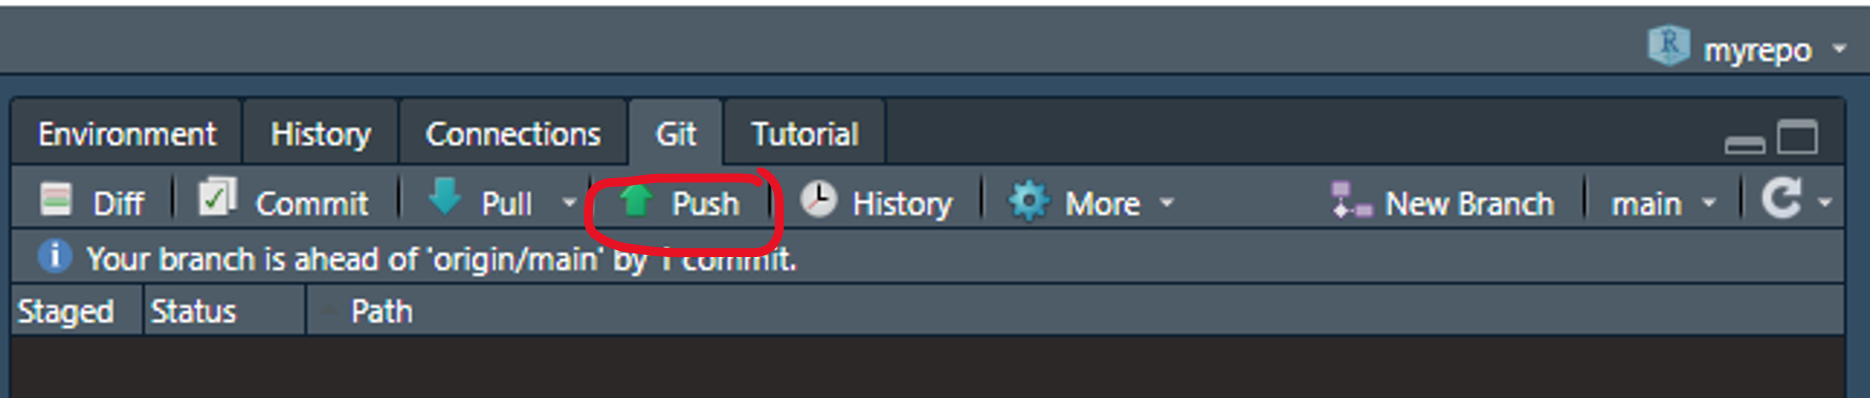
\includegraphics{assets/img/push.png}

\hypertarget{sync-local-copy-from-github-pull}{%
\subsection{Sync local copy from GitHub:
Pull}\label{sync-local-copy-from-github-pull}}

\begin{itemize}
\tightlist
\item
  In the GitHub repo main page\\
\item
  In the upper right corner of the Readme, click on the pencil
\item
  Add a line eg : ``Line added from GitHub.''
\item
  Click ``Commit changes.''
\item
  In RStudio click Pull on the Git pane
\item
  You should see the new line in the Readme
\end{itemize}

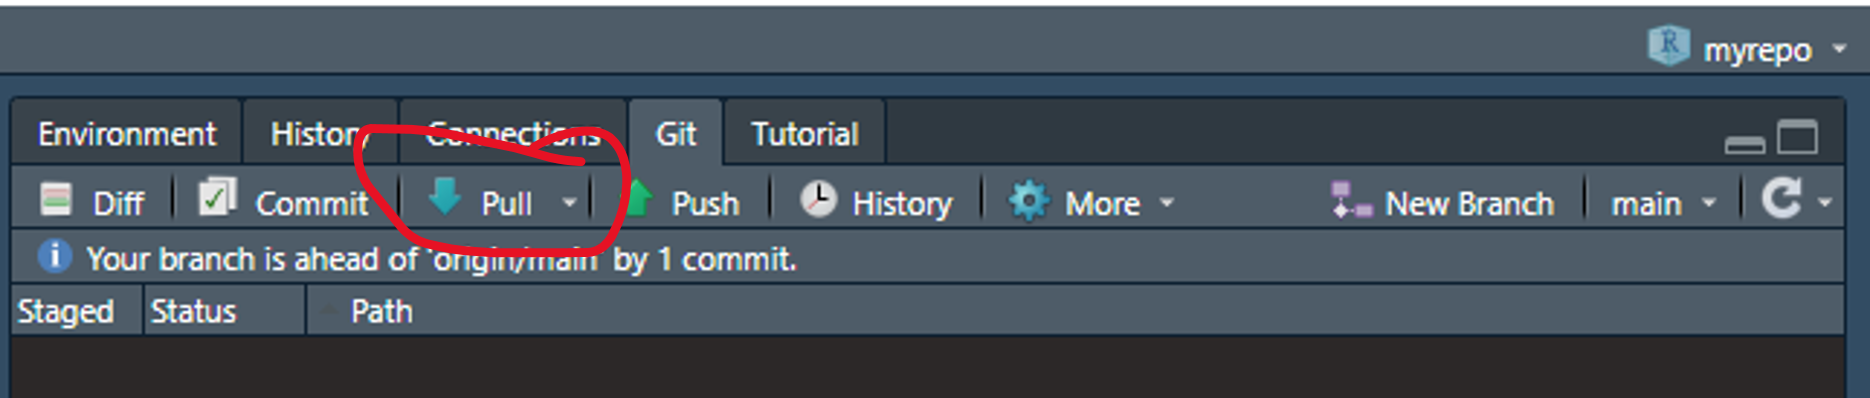
\includegraphics{assets/img/pull.png}

\hypertarget{add-an-existing-project-to-github}{%
\section{Add an existing project to
GitHub}\label{add-an-existing-project-to-github}}

\begin{itemize}
\tightlist
\item
  Create a new repo and Rstudio project in the same way as above
\item
  Simply copy all files into the newly created folder on your local
  computer
\item
  Stage and commit all files that you \textbf{want to store on GitHub}

  \begin{itemize}
  \tightlist
  \item
    Nothing sensitive ie passwords, keys etc (you can have a private
    repo if you are not ready to share code with the world)
  \item
    Probably not large datasets
  \item
    Use . gitignore to avoid git tracking things (more on this later)
  \end{itemize}
\end{itemize}

\emph{This is the simplest way to do it but there are more advanced,
more traditional git ways to do it:
\url{https://happygitwithr.com/existing-github-last.html}}

\hypertarget{issues-with-installation}{%
\section{Issues with installation}\label{issues-with-installation}}

If RStudio is not finding a git installation: + Restart RStudio and try
again + If still not working, run this in the windows command line:
\texttt{git\ -\/-exec-path} + Copy the path, then in RStudio click Tools
\textgreater{} Global Options \textgreater{} Git/SVN and set the Git
executable by clicking browse, pasting the path in the address bar and
selecting the git.exe file. + Restart RStudio again

See \url{https://happygitwithr.com/rstudio-see-git.html} for more
instructions on troubleshooting

\hypertarget{git-terminology-summary-1}{%
\section{Git terminology summary 1}\label{git-terminology-summary-1}}

\begin{itemize}
\tightlist
\item
  Repository (repo): Folder that contains a hidden .git file that tracks
  changes made to files in that folder. The folder can ``live'' on your
  local computer or a server like GitHub's. On GitHub the repository is
  also the web page where all the files are stored among other things
\item
  Push: Copy changes from your local version of the repo to the GitHub
  version
\item
  Pull: Copy changes from the GitHub version of the repo to your local
  version
\item
  Clone: make a copy of a git repository. By default in R studio this is
  connected to the GitHub version (called the remote or origin)
\item
  Commit: A marker that is kept in the git history and helps to
  incrementally track changes. Made useful by descriptive commit
  messages
\end{itemize}

\bookmarksetup{startatroot}

\hypertarget{using-git-and-github}{%
\chapter{Using Git and GitHub}\label{using-git-and-github}}

\hypertarget{tour-of-github-repository}{%
\section{Tour of GitHub repository}\label{tour-of-github-repository}}

\url{https://github.com/LandSciTech/caribouMetrics}

\hypertarget{code}{%
\subsection{Code}\label{code}}

\begin{itemize}
\tightlist
\item
  Top folder of repo.
\item
  Acts as landing page.
\item
  Displays the readme file.
\end{itemize}

\hypertarget{file-on-github}{%
\subsection{File on GitHub}\label{file-on-github}}

\begin{itemize}
\tightlist
\item
  Can view and edit code on GitHub.
\end{itemize}

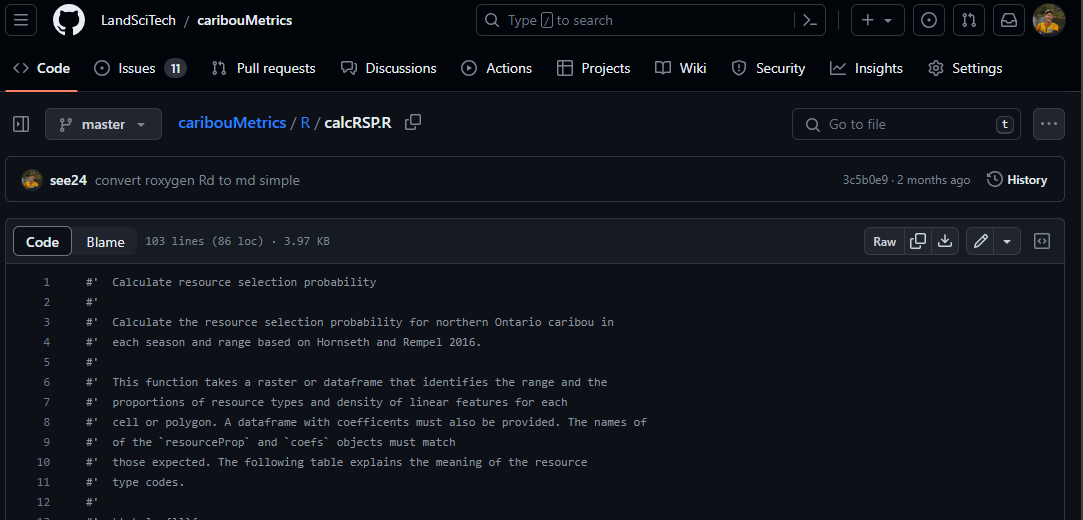
\includegraphics{assets/img/file.png}

\begin{itemize}
\tightlist
\item
  Can see what has changed over time.
\item
  History shows all commits that have affected the file.
\end{itemize}

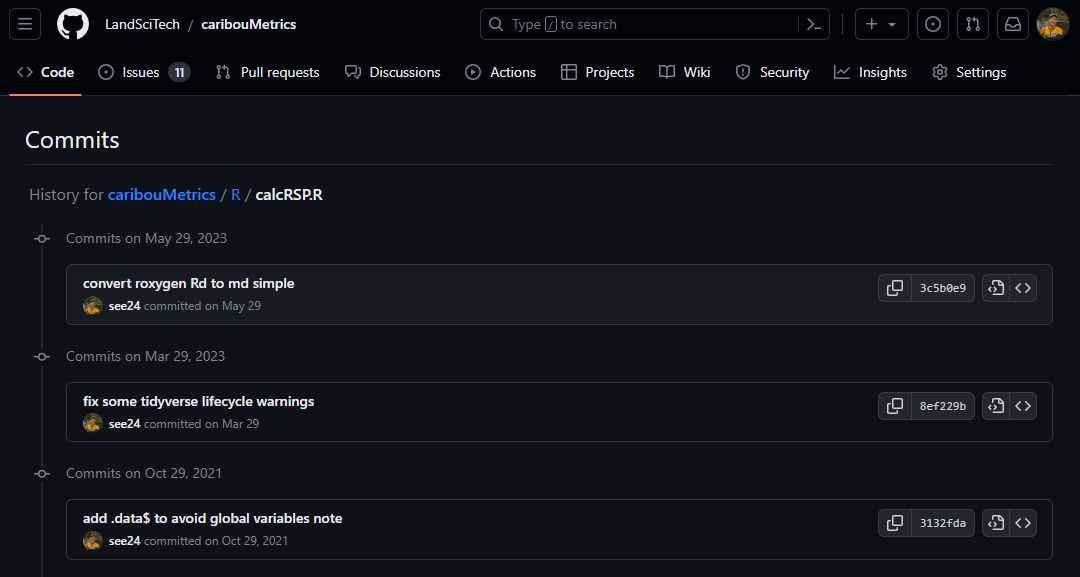
\includegraphics{assets/img/history.png}

\begin{itemize}
\tightlist
\item
  Blame shows for each line, who last edited, when, and the commit
  message.
\end{itemize}

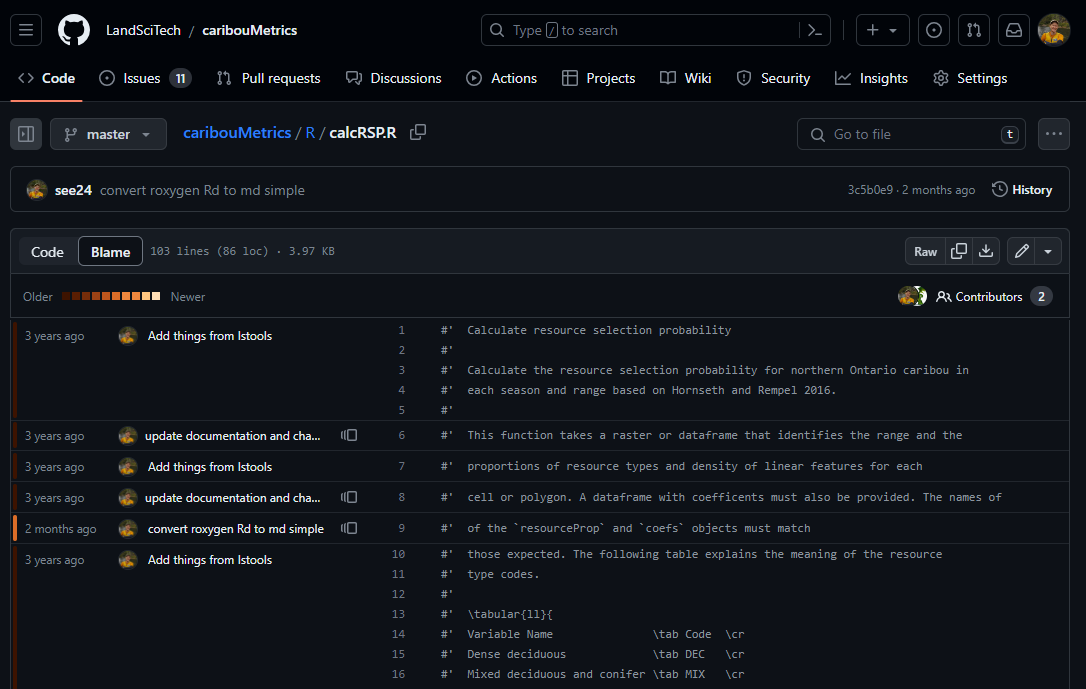
\includegraphics{assets/img/blame.png}

\hypertarget{viewing-a-commit}{%
\subsection{Viewing a commit}\label{viewing-a-commit}}

\begin{itemize}
\tightlist
\item
  Shows all files changed and highlights which parts changed.
\end{itemize}

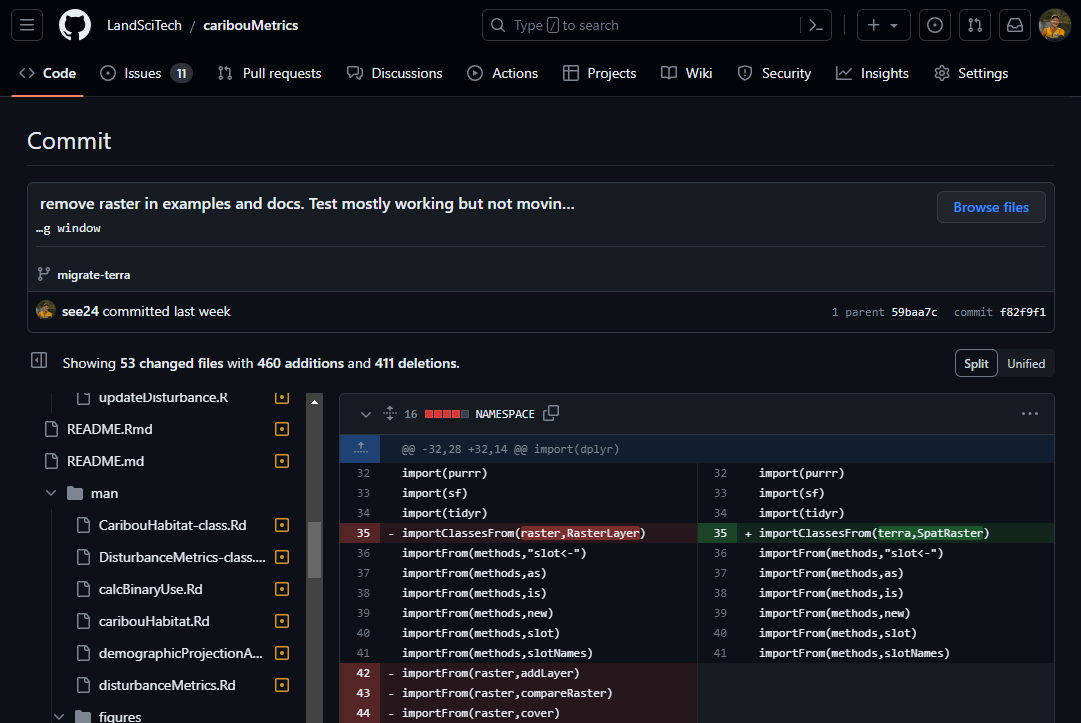
\includegraphics{assets/img/view_commit.png}

\begin{itemize}
\tightlist
\item
  Works for images too!
\end{itemize}

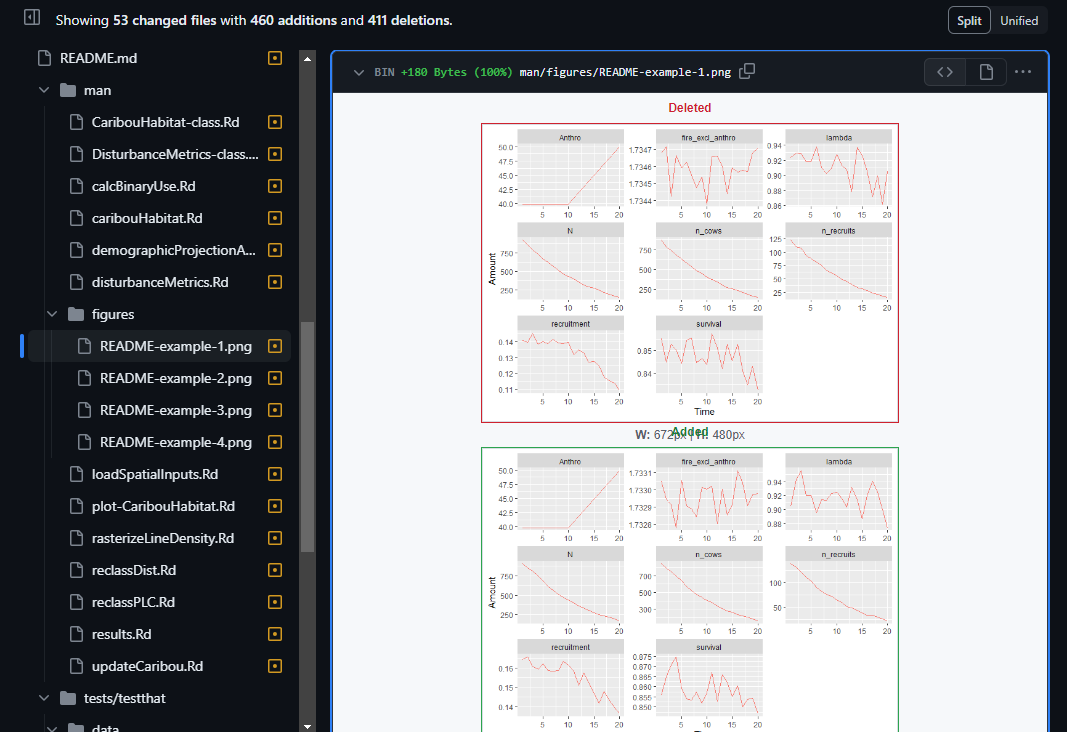
\includegraphics{assets/img/view_commit_img.png}

\hypertarget{issues}{%
\subsection{Issues}\label{issues}}

A place for tracking things that need to get done or reporting bugs or
unexpected results.

\begin{itemize}
\tightlist
\item
  Can be submitted by anyone with access to the repo.
\item
  Once they are dealt with they can be closed but are still kept.
\item
  If you are reporting a bug it is key to have a
  \href{https://stackoverflow.com/a/5963610/3277050}{minimum
  reproducible example} so others can see what you are seeing and try to
  help.
\item
  anywhere else on GitHub if you type \# and then the issue number it
  will automatically link to the issue. In a commit message this will
  link the commit to the issue so you can see what was changed to
  address it. Example
  \href{https://github.com/LandSciTech/caribouMetrics/issues/97}{here}.
\item
  Issues can also be used for To-do lists or project planning and can be
  tagged with a certain category or assigned to specific users.
\end{itemize}

\hypertarget{settings}{%
\subsection{Settings}\label{settings}}

Repository options and settings. There are a lot of complex options but
the most beginner relevant are:

\begin{itemize}
\tightlist
\item
  Changing repository visibility: Bottom of General section, usually
  changing to public once far enough along
\item
  Deleting repository: Bottom of General section, no going back,
  consider archiving if it is just out of date
\item
  Adding collaborators: under Access \textgreater{} Collaborators and
  teams, click add people and type their GitHub user name. Only needed
  for private repositories
\end{itemize}

\hypertarget{github-organiztions}{%
\subsection{GitHub Organiztions}\label{github-organiztions}}

\begin{itemize}
\tightlist
\item
  You can create an organization to group repos together and manage
  collaborators. For example:
\item
  \url{https://github.com/LandSciTech}
\item
  \url{https://github.com/PredictiveEcology}
\item
  \url{https://github.com/na-pops}
\end{itemize}

\hypertarget{daily-git-usage}{%
\section{Daily Git Usage}\label{daily-git-usage}}

\hypertarget{when-to-commit}{%
\subsection{When to commit}\label{when-to-commit}}

\begin{itemize}
\tightlist
\item
  Often!
\item
  But not too often!

  \begin{itemize}
  \tightlist
  \item
    Use ``Amend previous commit'' checkbox when you want to make sure to
    commit but aren't sure you are done yet
  \end{itemize}
\item
  Try to make each commit distinct and accomplish one thing. eg:

  \begin{itemize}
  \tightlist
  \item
    \texttt{Make\ data\ cleaning\ script}
  \item
    \texttt{Create\ exploratory\ plots}
  \item
    \texttt{Fix\ bug\ in\ data\ cleaning\ handling\ of\ dates}
  \item
    \texttt{Update\ exploratory\ plots\ with\ dates}
  \end{itemize}
\end{itemize}

\hypertarget{what-to-commit}{%
\subsection{What to commit}\label{what-to-commit}}

\begin{itemize}
\tightlist
\item
  Everything!

  \begin{itemize}
  \tightlist
  \item
    Git can track any file but it does a better job with raw text files
    (eg: .R, .Rmd, .html, .md, .py, .sh, .txt)
  \item
    For files like word docs or pdfs it can't track the content and
    tracks the whole file every time you make a change
  \end{itemize}
\item
  Except!:

  \begin{itemize}
  \tightlist
  \item
    Nothing sensitive ie passwords, keys etc (you can have a private
    repo if you are not ready to share code with the world but still
    don't store passwords)
  \item
    Probably not large datasets. I just keep these locally but would be
    better to have them on a shared drive and download them
    programmatically
  \end{itemize}
\item
  .gitignore: a file at the top level of git repo that tells git what
  not to track.

  \begin{itemize}
  \tightlist
  \item
    Uses regular expressions to match file or folder names or types.
  \item
    Example file:
    \url{https://github.com/LandSciTech/caribouMetrics/blob/master/.gitignore}
  \end{itemize}
\end{itemize}

\hypertarget{when-to-push}{%
\subsection{When to push}\label{when-to-push}}

\begin{itemize}
\tightlist
\item
  Fairly often. If you are working alone pushing is a way to back up
  your files. If you are collaborating it is a way to make your work
  available to others. If you don't push and then a collaborator makes
  changes to the same file it gets a bit tricky (but fixable).
\item
  Once you push you can't use the ``Amend previous commit'' trick
\item
  If you find yourself reluctant to push because you aren't ready for
  others to use your work consider making a branch (see below)
\end{itemize}

\hypertarget{when-to-pull}{%
\subsection{When to pull}\label{when-to-pull}}

\begin{itemize}
\tightlist
\item
  Ideally every day, or when a collaborator lets you know they pushed
\item
  Pulling often prevents getting out of sync with collaborators
\item
  Before pulling be sure to commit all your local work
\item
  Good practice to pull before pushing but git will normally warn you if
  you forget.
\end{itemize}

\hypertarget{merge-conflicts-in-pushpull}{%
\subsection{Merge conflicts in
Push/Pull}\label{merge-conflicts-in-pushpull}}

\begin{itemize}
\tightlist
\item
  If a collaborator pushed their changes after you last pulled you will
  need to pull before you can push. If your changes don't conflict git
  will automatically merge their changes with yours.
\item
  Merge conflicts: when a collaborator made changes that overlap your
  changes. Git can't automatically fit them together you have to review
  and pick the part to keep.
\end{itemize}

\hypertarget{resolving-merge-conflicts}{%
\subsection{Resolving merge conflicts}\label{resolving-merge-conflicts}}

This is a typical scenario with a merge conflict: ``Ah! I pulled at the
start of the day but then a collaborator pushed a change to the same
line and now when I try to push it says I have to pull first.''

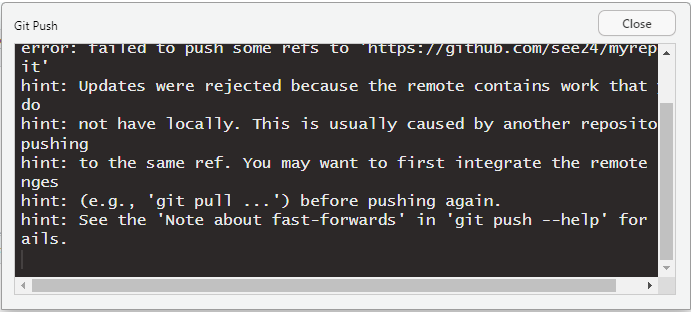
\includegraphics{assets/img/push_fail.PNG}

``And then when I pull I get merge conflicts!''

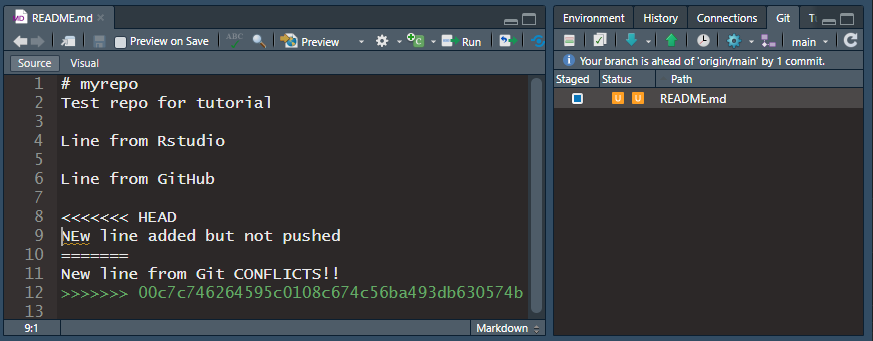
\includegraphics{assets/img/merge_conflict.png}

Not too hard to fix. Go through each file that has the orange U in the
Git pane. Find the location of the conflict. HEAD is your local version
and the alphanumeric string is the commit id for the remote version that
conflicts. Pick the one you want and delete all the marker lines
(\textless\textless\textless, === and
\textgreater\textgreater\textgreater). Then commit and continue on with
your work.

\hypertarget{avoiding-merge-conflicts}{%
\subsection{Avoiding merge conflicts}\label{avoiding-merge-conflicts}}

\begin{itemize}
\tightlist
\item
  Pull regularly
\item
  Keep in touch with collaborators so you are not working on the same
  lines at the same time.
\item
  Use a branch
\end{itemize}

\hypertarget{tools-for-collaboration}{%
\section{Tools for Collaboration}\label{tools-for-collaboration}}

\hypertarget{write-good-code}{%
\subsection{Write good code}\label{write-good-code}}

Writing good code with a consistent style, literate naming and comments
to explain decisions goes a long way to improving collaboration. It is
also required that your code runs on your collaborators computer without
significant modifications. See the
\href{https://github.com/LandSciTech/R-Resources/wiki/Minimum-requirements-for-\%22good\%22-code}{LandSciTech/R-Resources
Wiki} for some ideas on how to write good code.

\hypertarget{branches}{%
\subsection{Branches}\label{branches}}

\begin{itemize}
\tightlist
\item
  A stream of commits that diverges from the main stream until it is
  ready to re-join.
\item
  Helpful for starting a new version of something while making sure
  others can keep using the old version
\item
  Example we want to convert some functions used in a paper to become an
  R package but Josie is working on writing the paper and needs the old
  version to keep working. I make a branch where I re-arrange everything
  into a package. If Josie makes changes to the main branch that affect
  the functions I can see those and merge them into my branch.
\item
  See \url{https://happygitwithr.com/git-branches.html\#\#git-branches}
  for how to manage branches with the command line but it can also be
  done through the Rstudio IDE and GitHub for the most part.
\end{itemize}

\hypertarget{make-a-new-branch-in-rstudio}{%
\subsubsection{Make a new branch in
RStudio}\label{make-a-new-branch-in-rstudio}}

\begin{itemize}
\tightlist
\item
  Click New Branch in the Git pane
\end{itemize}

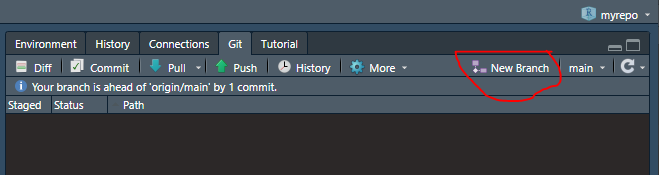
\includegraphics{assets/img/new_branch.png}

\begin{itemize}
\tightlist
\item
  Give it a name using dashes or underscores for spaces and no special
  characters. The ``Remote'' is the GitHub version of the repository,
  almost always leave the default. ``Sync branch with remote'' will also
  create the branch on GitHub which we typically want. Click ``Create''
\end{itemize}

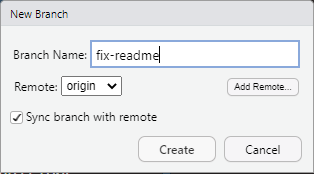
\includegraphics{assets/img/new_branch_name.png}

\begin{itemize}
\tightlist
\item
  Make a change, save, commit and push as usual.
\item
  To change back to the main branch click the dropdown beside the ``New
  Branch'' button and under ``Local Branches'' select ``main''. In git
  this is called ``checking out'' the branch.
\end{itemize}

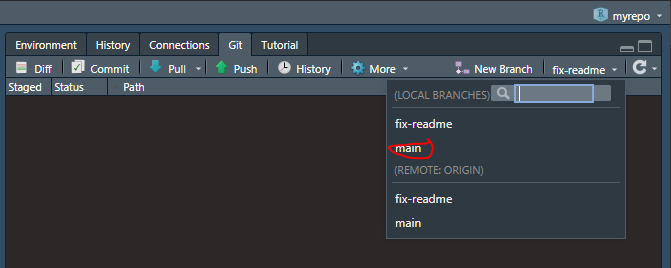
\includegraphics{assets/img/change_branch.png}

\hypertarget{merge-the-branch-back-into-main-with-a-pull-request}{%
\subsubsection{Merge the branch back into main with a Pull
Request}\label{merge-the-branch-back-into-main-with-a-pull-request}}

\begin{itemize}
\tightlist
\item
  Once you are ready to incorporate the changes in your branch back into
  the main code stream you ``merge'' your branch with the main branch.
\item
  The easiest way to do that is on GitHub. Once you have made commits on
  your branch and pushed go to the repo on GitHub
\item
  On the GitHub repo page select the new branch from the drop down, then
  click Contribute \textgreater{} Open pull request
\end{itemize}

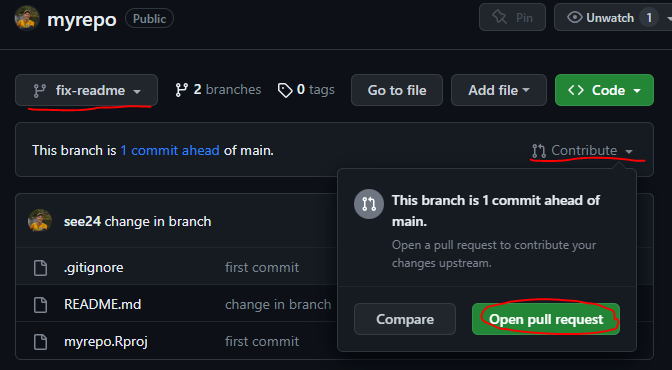
\includegraphics{assets/img/make_PR.png}

\begin{itemize}
\tightlist
\item
  You can give the pull request a descriptive name and add comments to
  explain what your are trying to do or link to issues that are being
  addressed. Then create the pull request.
\item
  The pull request (PR) is a page that summarizes the changes you
  propose to make to the main branch. It includes the list of commits in
  the branch since it diverged from main and the diffs for files that
  have changed. Collaborators can leave comments on the PR and discuss
  it or add new commits before it is merged.
\item
  PRs are the main way you can contribute to open source projects, and
  in that case the owner of the project will get the final decision
  whether to merge your changes into the main branch.
\item
  If there are no merge conflicts and you have the authority to commit
  to the repos main branch you can click ``Merge pull request'' to merge
  your branch with main branch. Then you can delete the branch if it is
  no longer needed. On your local Rstudio session you will need to
  change back to the main branch and pull so that the changes are
  reflected in your local copy of the main branch.
\item
  Branches don't really prevent merge conflicts. But they do allow you
  to decide when you want to deal with reconciling your branch and the
  main branch so you can be more intentional about it. If the same parts
  of the code are changed in the main branch and your new branch you
  have to decide manually which one to keep by resolving the merge
  conflicts as described above. GitHub provides an editor to resolve
  conflicts online. In some situations the conflicts are too complex to
  resolve online and the merge must be done from the command line.
  GitHub provides instructions if this happens.
\end{itemize}

\hypertarget{merge-changes-from-main-into-your-branch}{%
\subsubsection{Merge changes from main into your
branch}\label{merge-changes-from-main-into-your-branch}}

\begin{itemize}
\tightlist
\item
  Sometimes changes are made in main (or any other branch) that you want
  to include in your branch without incorporating the changes in your
  branch into main
\item
  To do this you merge the main branch with yours. On GitHub if you go
  to your branch and click the ``This branch is x commits behind main''
  url it will open a PR for merging main into your branch.
\end{itemize}

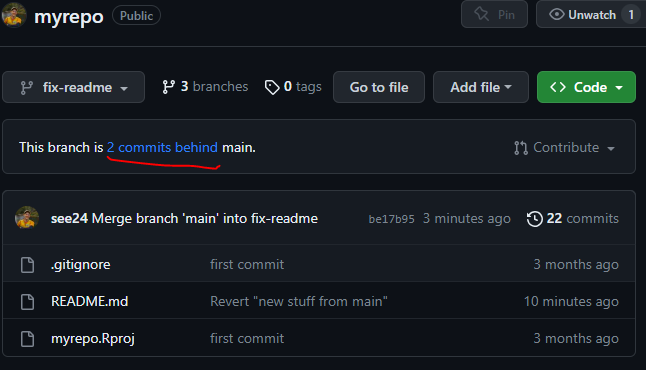
\includegraphics{assets/img/update_branch_PR.png}

\begin{itemize}
\tightlist
\item
  A PR is often unnecessary for merging main into your branch, because
  most times your collaborators don't need to know about it. To avoid
  this you can use the command line to do the merge.
\item
  In RStudio on the Console pane click the Terminal tab. This will open
  a command line where you can type git commands.
\item
  Make sure you are in your branch that you want to merge into. Then
  type: \texttt{git\ merge\ main}
\end{itemize}

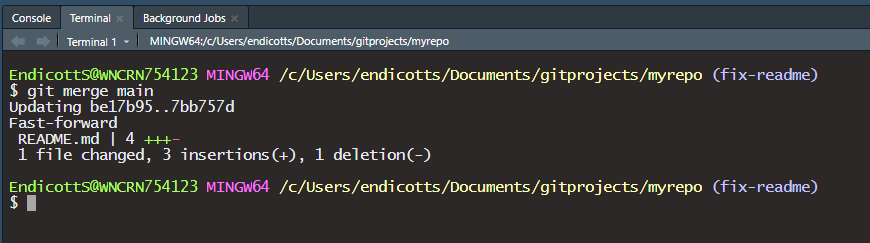
\includegraphics{assets/img/merge_cmd.png}

\hypertarget{forks}{%
\subsection{Forks}\label{forks}}

\begin{itemize}
\item
  A fork is a copy of another repository which is used to contribute to
  an open source project that you do not have permission to edit, or to
  simply make a copy and edit as you wish from there but with an
  acknowledgement that you used another repo as a starting point.
\item
  you can create a fork on GitHub by clicking the fork button in the top
  right of all GitHub repos or with the usethis command below which will
  also set up useful default settings. See
  \href{https://happygitwithr.com/fork-and-clone.html\#fork-and-clone-create-from-github}{here}
  for more details.
\end{itemize}

\begin{Shaded}
\begin{Highlighting}[]
\NormalTok{usethis}\SpecialCharTok{::}\FunctionTok{create\_from\_github}\NormalTok{(}
  \StringTok{"https://github.com/OWNER/REPO"}\NormalTok{,}
  \AttributeTok{destdir =} \StringTok{"\textasciitilde{}/path/to/where/you/want/the/local/repo/"}\NormalTok{,}
  \AttributeTok{fork =} \ConstantTok{TRUE}
\NormalTok{)}
\end{Highlighting}
\end{Shaded}

\hypertarget{git-terminology-summary-2}{%
\section{Git Terminology Summary 2}\label{git-terminology-summary-2}}

\begin{itemize}
\tightlist
\item
  Merge: Combine two versions of a file. These can be the local and
  GitHub (remote) copies or two different branches.
\item
  Conflict: When merging can't be done automatically because two
  versions of the code have edited the same part of a file.
\item
  Branch: A copy of the code that you want to keep separate from the
  main code at least for a time.
\item
  Pull request: A special GitHub page that shows what will be added to
  the main branch when another branch is merged.
\item
  Fork: A copy of a repository that you don't own. Used for contributing
  to open source projects.
\end{itemize}

\bookmarksetup{startatroot}

\hypertarget{intermediate-git}{%
\chapter{Intermediate Git}\label{intermediate-git}}

\hypertarget{time-travel}{%
\section{Time travel}\label{time-travel}}

One of the key benefits of using version control is the ability to go
backwards and see what a project looked like at a previous time point.

\hypertarget{individual-files}{%
\subsection{Individual files}\label{individual-files}}

As mentioned in the previous
\href{https://landscitech.github.io/Github_tutorial/git-basics.html\#file-on-github}{chapter}
you can see the changes to a file using the History or Blame buttons on
GitHub. You can also view the History of your repo in RStudio by
clicking ``History'' in the Git Pane. This will show you a Window with
all your commits and you can select one to see what it changed. You can
also click ``View file @ SHA'' to see the full file at that point in
history, which you can then save or run as you see fit.

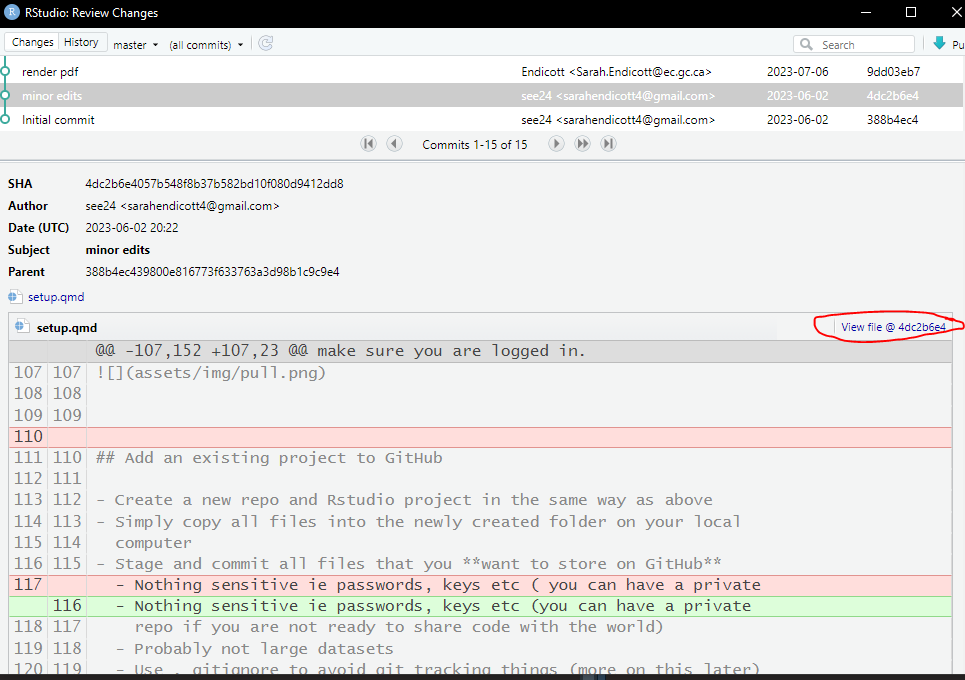
\includegraphics{assets/img/RS_history.PNG}

\hypertarget{whole-repository}{%
\subsection{Whole repository}\label{whole-repository}}

You can also look at the whole repository at a previous time point. On
GitHub on the Commits page you can click the ``\textless\textgreater{}''
button to browse the repository at that point in the commit history.
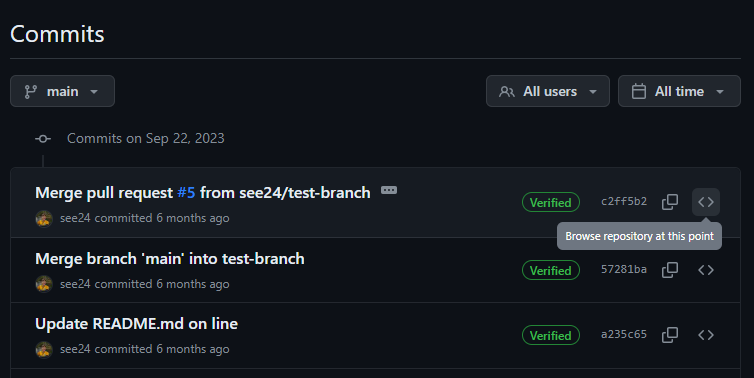
\includegraphics{assets/img/view_repo_at_point.PNG.PNG}

On your local computer you can change the files back to how they were at
a particular point in history using the git checkout command. This is
the same command used to switch branches. You can use a specific commit
name or move a certain number of commits back from the current status
(HEAD).

If you try to do this with uncommited changes you will get an error
saying you must first commit your changes.

Example commands:

\begin{itemize}
\tightlist
\item
  \texttt{git\ switch\ -d\ HEAD\^{}}: go to previous commit
\item
  \texttt{git\ switch\ -d\ HEAD\textasciitilde{}3}: go back three
  commits
\item
  \texttt{git\ switch\ -d\ 4959f4d}: go to the commit with the id
  ``4959f4d''
\end{itemize}

When do this you are in `detached HEAD' state (-d is short for
--detach). You can look around, make experimental changes and commit
them, and you can discard any commits you make in this state without
impacting any branches by switching back to a branch.

If you want to create a new branch to retain commits you create, you may
do so (now or later) by using -c with the switch command. Example:

\texttt{git\ switch\ -c\ \textless{}new-branch-name\textgreater{}}

When you are done you can go back to the most recent commit on the
master branch (or other branch) with \texttt{git\ switch\ master}.

Note: \texttt{switch} is a newer git command so you will see older help
docs and such use \texttt{checkout} for this task. \texttt{switch} was
added because \texttt{checkout} does a lot of different things and is
confusing to new users so I am using \texttt{switch} here.

\hypertarget{changing-history}{%
\section{Changing history}\label{changing-history}}

At this stage we haven't actually changed anything in our repository. If
you can use the above strategies to figure out where something went
wrong and then fix it in a new commit that is probably the easiest
thing. If you want to undo all the changes after a particular commit you
can use \texttt{revert} or \texttt{reset}. \texttt{revert} is the safer
option, it reverse engineers the changes from a previous commit and then
adds a new commit to the repository with the changes removed. This is
safe because it keeps the whole history so if you then decided to undo
the undo you still have the commit from before you called
\texttt{revert}. This is the best solution for changes that have been
pushed to GitHub. \texttt{reset} can be used to erase all the commits
between the current commit and the commit given to the command. There
are several options that can be applied to it which affect what happens
to the files that were edited in those intervening commits. With
\texttt{reset\ -\/-hard} the changes to the files are also removed, this
cannot be undone so only use it if you are very sure you want to get rid
of all changes made. \texttt{reset\ -\/-mixed} will delete any new
commits but will keep the changes to the files as uncommitted changes in
your local file system. Resetting is problematic if you already pushed
the commit to GitHub because the version of the repository on GitHub has
the commit and thinks you are missing something so it won't let you push
easily. That is why you should only use \texttt{revert} for commits that
have been pushed.

\hypertarget{worked-example-of-reset-and-revert.}{%
\subsection{Worked example of reset and
revert.}\label{worked-example-of-reset-and-revert.}}

\bookmarksetup{startatroot}

\hypertarget{miscellaneous-tips-and-tricks}{%
\chapter{Miscellaneous tips and
tricks}\label{miscellaneous-tips-and-tricks}}

\hypertarget{easy-extensions}{%
\section{Easy Extensions}\label{easy-extensions}}

\begin{itemize}
\tightlist
\item
  Making a repo work like a simple website
  \url{https://happygitwithr.com/workflows-browsability.html\#\#workflows-browsability}
\item
  Installing a Git Client
  \url{https://happygitwithr.com/git-client.html\#\#git-client}
\item
  Good default folder structure and setup for a typical analysis
  project: \url{https://frbcesab.github.io/rcompendium/index.html}
\end{itemize}

\hypertarget{advanced-uses}{%
\section{Advanced Uses}\label{advanced-uses}}

\begin{itemize}
\tightlist
\item
  Host a website:
  \url{https://www.emilyzabor.com/tutorials/rmarkdown_websites_tutorial.html}
\item
  Use GitHub Actions for continuous integration:
  \url{https://beamilz.com/posts/series-gha/2022-series-gha-1-what-is/en/}
\item
  Using GitHub to manage frequently updated data:

  \begin{itemize}
  \tightlist
  \item
    \url{https://doi.org/10.1371/journal.pbio.3000125}\strut \\
  \item
    \url{https://www.updatingdata.org/githubactions/}
  \item
    \url{https://doi.org/10.1111/2041-210X.13982}
  \end{itemize}
\end{itemize}

\bookmarksetup{startatroot}

\hypertarget{references}{%
\chapter*{References}\label{references}}
\addcontentsline{toc}{chapter}{References}

\markboth{References}{References}

\href{https://happygitwithr.com/index.html}{Happy Git and GitHub for the
useR} by Jennifer Bryan ::: \{\#refs\} :::



\end{document}
